\documentclass[margin=5mm]{standalone}
\usepackage{tikz}
\usetikzlibrary{matrix,calc}

\usepackage{amsfonts, 
			amssymb, 
			amsmath, 
            graphicx}


\DeclareMathAlphabet\mathbfcal{OMS}{cmsy}{b}{n}

\begin{document}
\begin{tikzpicture}[every node/.style={anchor=north east,fill=white,minimum width=1.4cm,minimum height=7mm}]

\draw [red,dashed] (-3.4, -2.7) rectangle (0.2, 0.3);
\node[inner sep=0pt] (fMRI) at (0, 0) {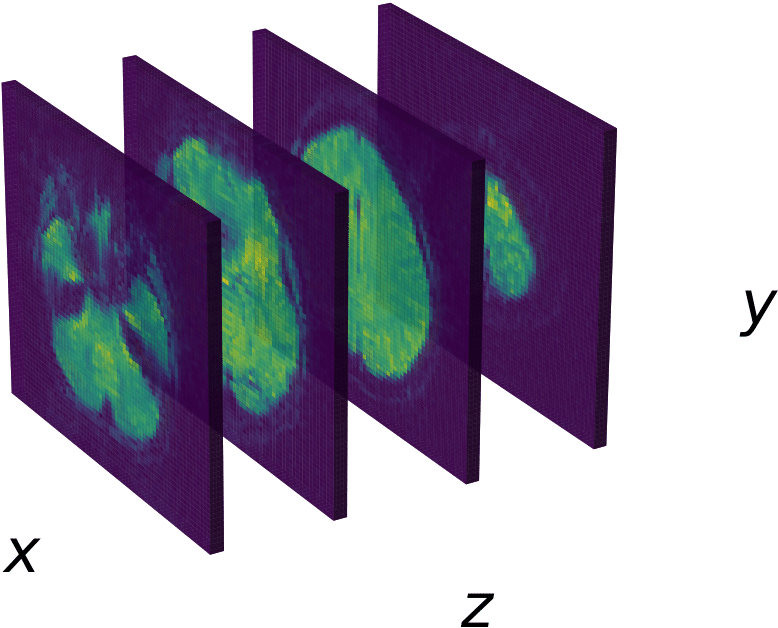
\includegraphics[width=.25\textwidth]{fMRI.png}};

\node [below, opacity=0, text opacity=1] at (0.6, -1) {$\otimes$};

\draw [green, dashed] (1, -2.7) rectangle (2.05, 0.3);
\node [below, opacity=0, text opacity=1] at (1.5, -1) {time};

\node [below, opacity=0, text opacity=1] at (2.45, -1) {$\otimes$};

\draw [blue, dashed] (2.9, -2.7) rectangle (6.5, 0.3);
\node[inner sep=0pt] (subjects) at (6.2, -0.2) {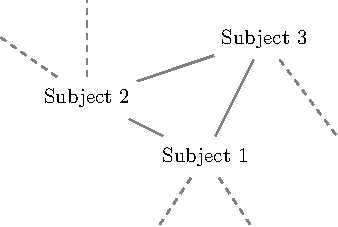
\includegraphics[width=.25\textwidth]{fMRI_Subjects_Diagram.pdf}};

\node [below, opacity=0, text opacity=1] at (6.9, -1) {$\otimes$};

\draw [orange, dashed] (7.4, -2.7) rectangle (10.5, 0.3);
\node[inner sep=0pt] (stimuli) at (10.3, -0.2) {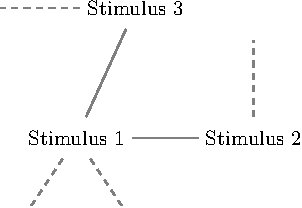
\includegraphics[width=.22\textwidth]{fMRI_Stimuli_Diagram.pdf}};





% \node [right,opacity=0,text opacity=1] at (-11.8,-3.0) {$n_2$};
% \node [right,opacity=0,text opacity=1] at (-12.2,-2.3) {$n_3$};

% \draw [-stealth](-12.5,-3) -- (-12.5,-4);
% \draw [-stealth](-12.5,-3) -- (-11.5,-3);
% \draw [-stealth](-12.5,-3) -- (-11.8,-2.5);



% \matrix (mA) [draw,matrix of math nodes]
% {
% (1,1,3) & (1,2,3) & (1,3,3) & (1,4,3) \\
% (2,1,3) & (2,2,3) & (2,3,3) & (2,4,3) \\
% (3,1,3) & (3,2,3) & (3,3,3) & (3,4,3) \\
% (4,1,3) & (4,2,3) & (4,3,3) & (4,4,3) \\
% };

% \matrix (mB) [draw,matrix of math nodes] at ($(mA.south west)+(3.5,1.5)$)
% {
% (1,1,2) & (1,2,2) & (1,3,2) & (1,4,2) \\
% (2,1,2) & (2,2,2) & (2,3,2) & (2,4,2) \\
% (3,1,2) & (3,2,2) & (3,3,2) & (3,4,2) \\
% (4,1,2) & (4,2,2) & (4,3,2) & (4,4,2) \\
% };

% \matrix (mC) [draw,matrix of math nodes] at ($(mB.south west)+(3.5,1.5)$)
% {
% (1,1,1) & (1,2,1) & (1,3,1) & (1,4,1) \\
% (2,1,1) & (2,2,1) & (2,3,1) & (2,4,1) \\
% (3,1,1) & (3,2,1) & (3,3,1) & (3,4,1) \\
% (4,1,1) & (4,2,1) & (4,3,1) & (4,4,1) \\
% };

% \draw[dashed](mA.north east)--(mC.north east);
% \draw[dashed](mA.north west)--(mC.north west);
% \draw[dashed](mA.south east)--(mC.south east);

% \node [right,opacity=0,text opacity=1] at (1.3,-1.5) {$\text{vec}_{\text{RM}}(\cdot)$};
% \draw [-stealth, line width=2pt](1,-1.9) -- (3,-1.9);

% \node [right,opacity=0,text opacity=1] at (1.3,-3.5) {$\text{ten}_{\text{RM}}(\cdot)$};
% \draw [stealth-, line width=2pt](1,-3.9) -- (3,-3.9);

% \node [right,opacity=0,text opacity=1,scale=1.3] at (4.3,0.7) {$\mathbf{y}$};
% \node [right,opacity=0,text opacity=1,scale=1.3] at (-3.8,0.7) {$\mathbfcal{Y}$};



% \matrix (mD) [draw, matrix of math nodes] at (6, -0.1)
% {
% (1,1,1) \\
% (1,1,2) \\
% (1,1,3) \\
% (1,2,1) \\
% \vdots \\
% (2,1,1) \\
% \vdots \\
% (4,4,3)  \\
% };

\end{tikzpicture}
\end{document}